\chapter{Część praktyczna}


\begin{figure}[!ht]
    \centering
    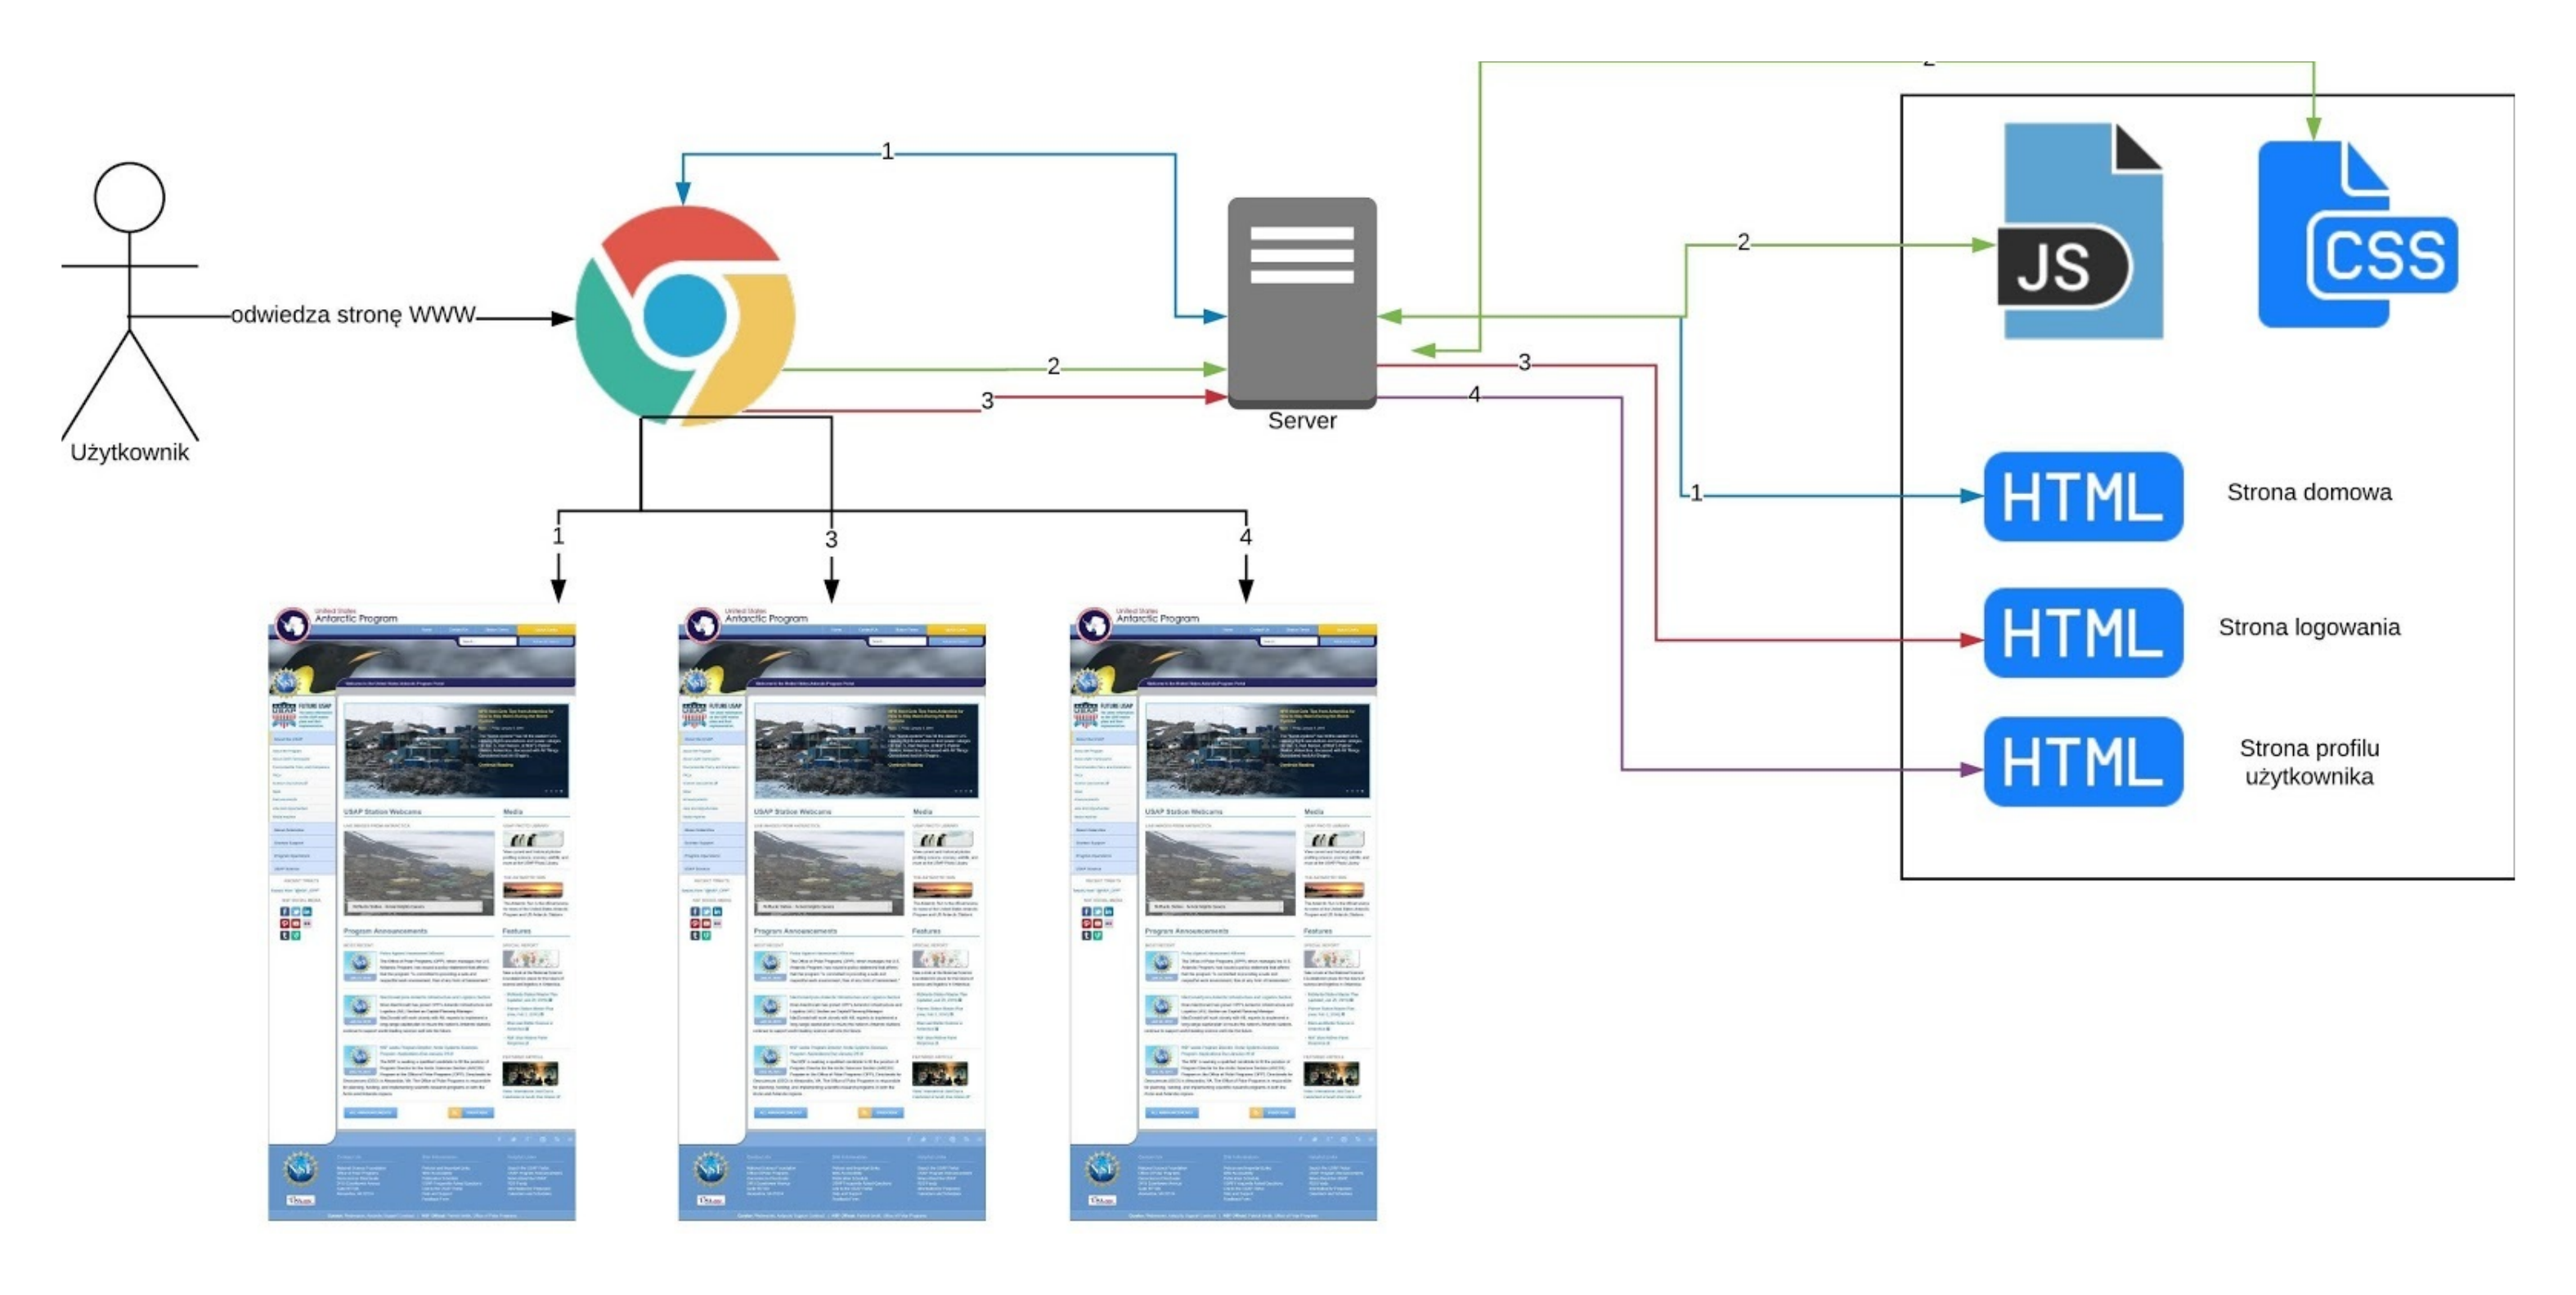
\includegraphics[width=12cm]{rysunek_7.png}
    \caption{Ilustracja przedstawiająca cykl życia statycznej strony internetowej}
    \label{fig:rysunek_7}
\end{figure}

\begin{figure}[!ht]
    \centering
    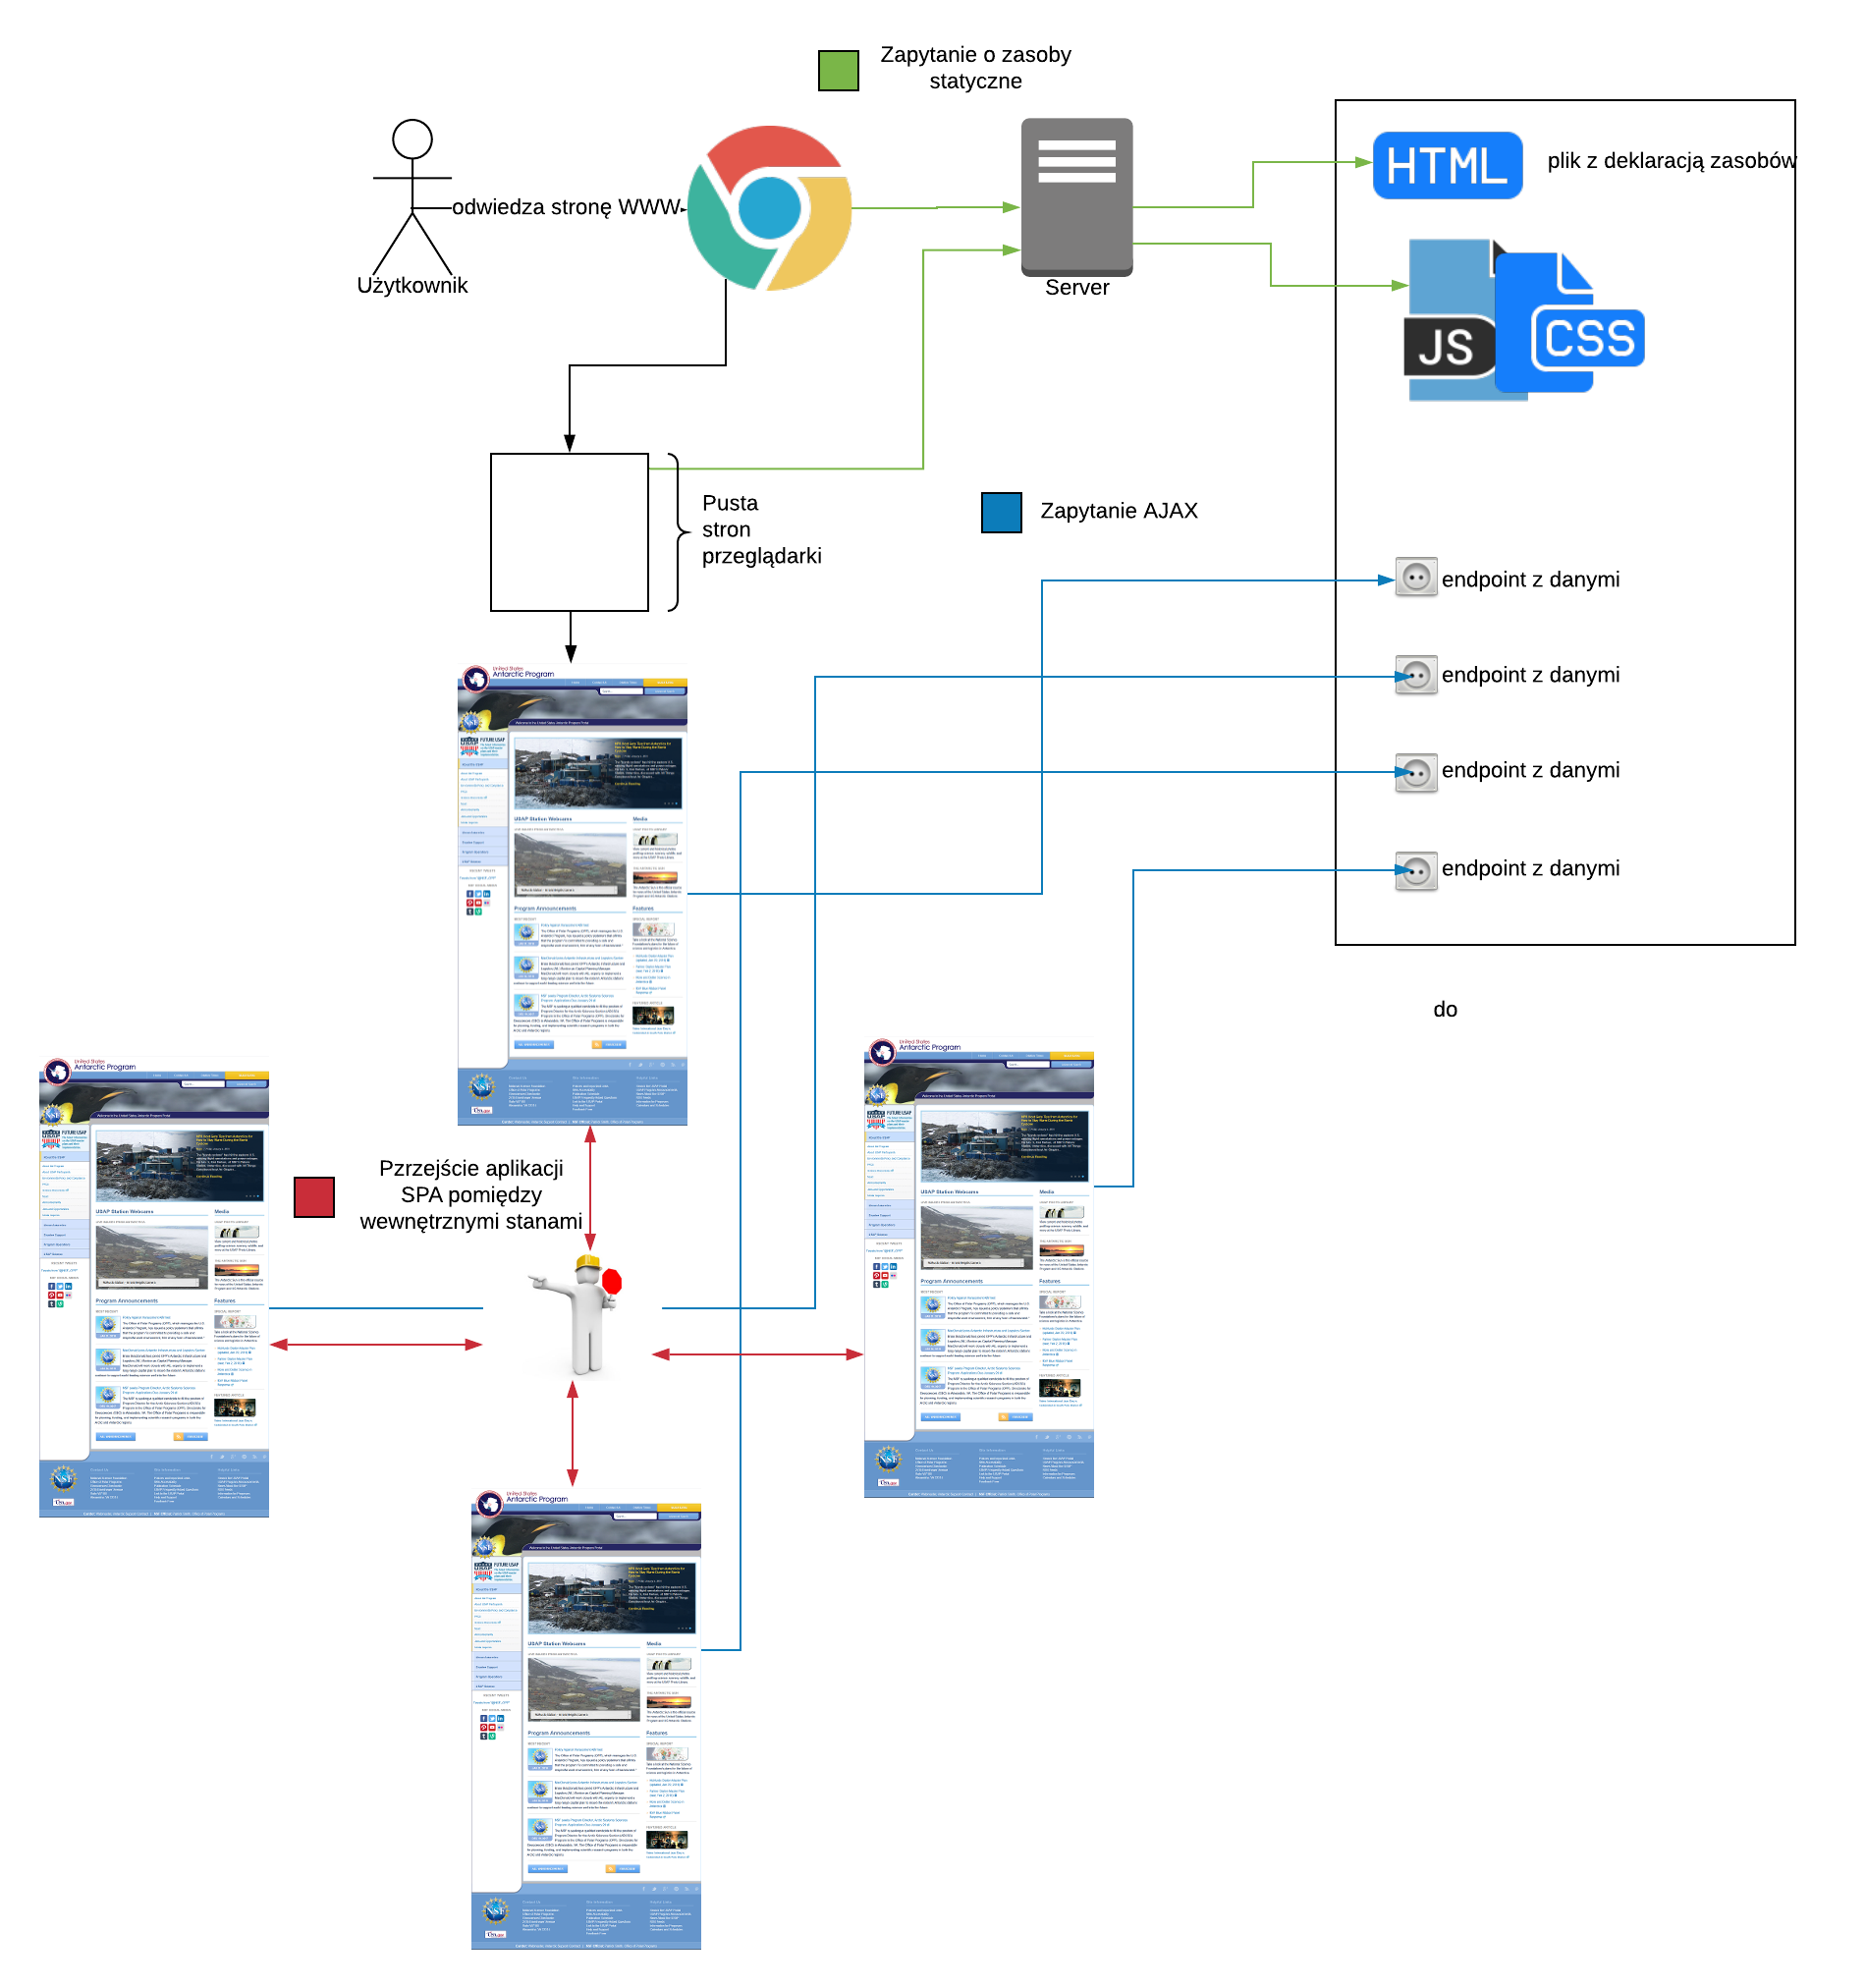
\includegraphics[width=12cm]{rysunek_8.png}
    \caption{Ilustracja przedstawiająca cykl działania aplikacji SPA}
    \label{fig:rysunek_8}
\end{figure}

\begin{figure}[!ht]
    \centering
    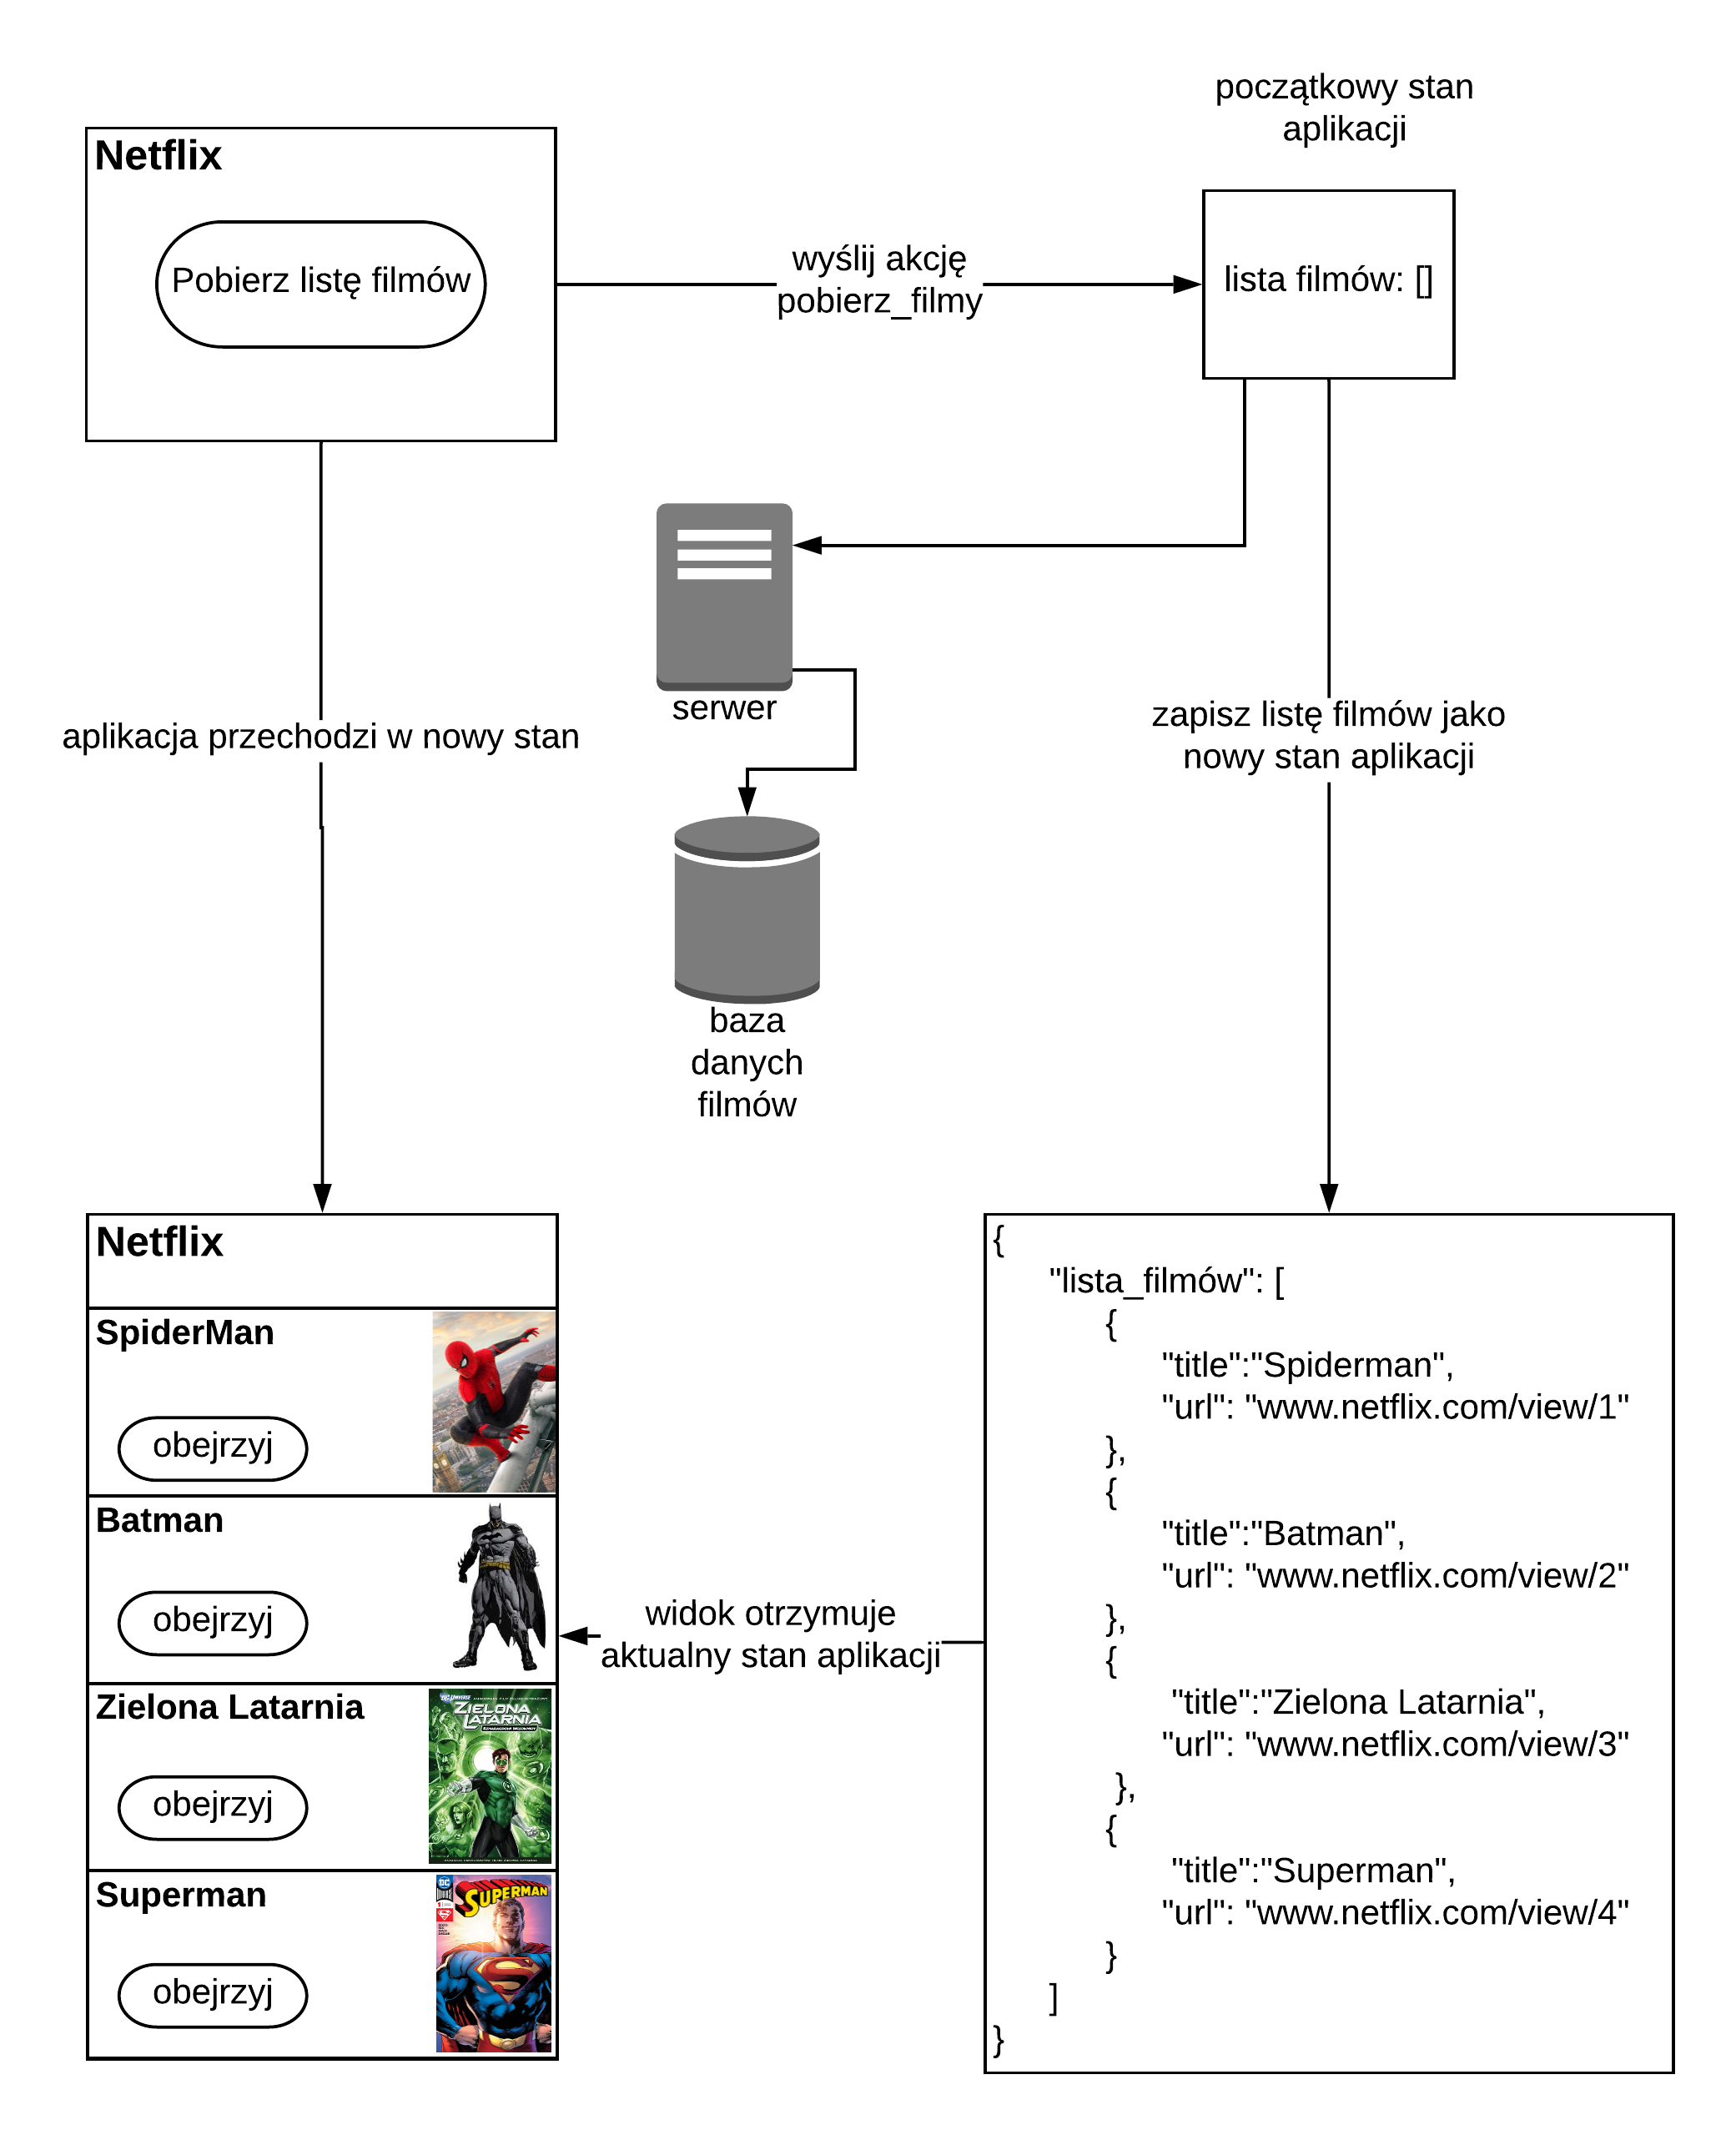
\includegraphics[width=12cm]{rysunek_9.png}
    \caption{Grafika przedstawiająca mechanizm działania aplikacji dynamicznych}
    \label{fig:rysunek_9}
\end{figure}

\begin{figure}[!ht]
    \centering
    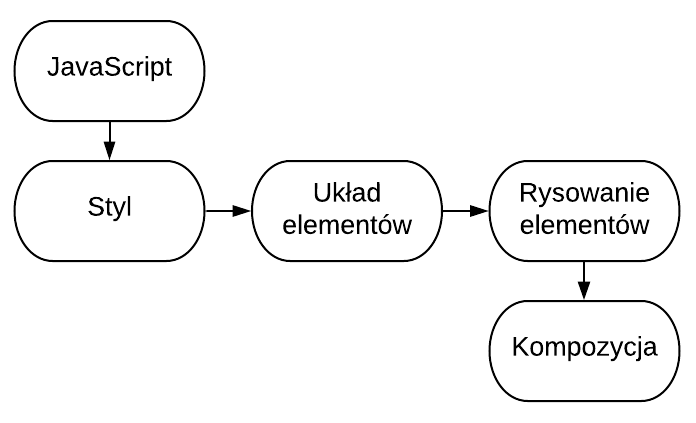
\includegraphics[width=12cm]{rysunek_10.png}
    \caption{Grafika przedstawiająca kolejność faz renderowania w przeglądarce}
    \label{fig:rysunek_10}
\end{figure}


%czyści puste strony
\let\cleardoublepage\clearpage